\chapter[Methods]%
{Methods}

\section{Introduction}

Firstly, differential gene expression analysis was performed. Then, feature reduction of the base-level modification information obtained from ONT episequencing was carride out. Finally, we trained a predictive model using the reduced feature matrix.

\begin{figure}[ht]
        \begin{center}
            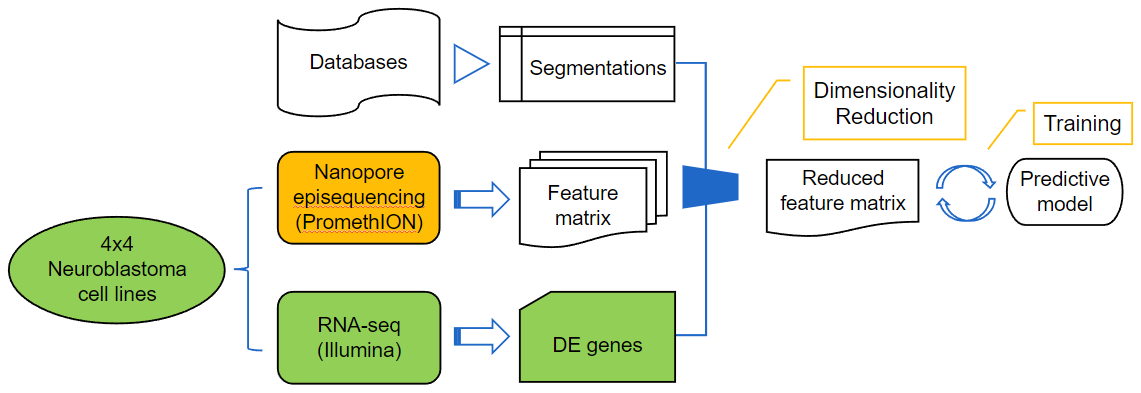
\includegraphics[width = \textwidth]{Fig/overview_temp.png}
        \end{center}
        \caption{Overview workflow.}
\end{figure}

\section{Samples}

To start off, expression data from 4 cell lines was gathered, namely 2 resistant and 2 sensitive neuroblastoma cell lines in quadruplicate (16 samples in total). These cell lines were characterized in terms of sensitivity towards ferroptosis beforehand experimentally. Furthermore, neuroblastoma is highly iron addicted which makes it exceptionally vulnerable to ferroptosis \citep{nb_iron}. Metadata for each cell line can be found in Table \ref{tab:cellline_meta}.

\begin{table}[!ht]
    \centering
    \begin{adjustbox}{width=\textwidth}
    \begin{tabular}{|l|l|l|l|l|}
    \hline
        \bfseries Cell Line & \bfseries Tumor Type & \bfseries Ferroptosis Sensitivity & \bfseries Gender & \bfseries Age (months) \\ \hline
        IMR-32 & Neuroblastoma & Sensitive & Male & 13 \\ \hline
        SH-EP & Neuroblastoma & Sensitive & Female & 48 \\ \hline
        SH-SY5Y & Neuroblastoma & Resistant & Female & 48 \\ \hline
        SK-N-BE(2)-C & Neuroblastoma & Resistant & Male & 26 \\ \hline
    \end{tabular}
    \end{adjustbox}
    \caption{Cell Line Metadata}
    \label{tab:cellline_meta}
\end{table}

\section{Gene Whitelist}

Genes thought to be associated with ferroptosis were compiled into a custom gene whitelist. The full list can be found in Appendix X.

\section{RNA-seq}



\section{ONT-seq}

For the episequencing, a PromethION nanopore sequencing device based at OHMX.bio was used, containing 24 channels per flow cell. PromethION offers a significantly higher number of channels compared to other ONT platforms like MinION and GridION. This high channel count enhances the platform's capacity for parallel sequencing.

From the whitelist, a BED file was constructed. Additionally, each gene was extended by 15kB, after which overlapping genes were joined together.

Library prep involved following protocol SQK-NBD114.24, describing how to carry out native barcoding of \ac{gDNA} using the Native Barcoding Kit 24 V14. Raw signal data in pod5 format was basecalled with a SUP model and 5(h)mC calling in CG context using GPU hardware on a GridION unit installed at OHMX.bio, and then subsequently demultiplexed. The basecalling model was set to fast, with the intent of making the decision of whether to reverse the voltage of the pore as fast as possible. The resulting unmapped bam files were then aligned against a reference genome, and finally sorted and indexed using SAMtools \citep{samtools}.

\section{Differential Gene Expression Analysis}



\section{Feature Engineering}



\section{Feature Reduction}

Since the episequencing returns many thousands of individual detected CpGs by locus, the number of features in our model will be staggering if used in its raw form. The first reduction of features will be actualized by bundling CpG sites into regions (e.g. CpG islands). A second dimensionality reduction will also be performed based on drivers derived from expression data, to remove sites or regions without genes that are differentially expressed by sensitivity.
